\documentclass[12pt,a4paper,oneside]{report}
\usepackage[hyphens]{url} % Permette la sillabazione degli URL

% Pacchetti necessari
\usepackage[italian]{babel} % Per la lingua italiana
\usepackage[T1]{fontenc} % Codifica dei font
\usepackage[utf8]{inputenc} % Codifica del file
\usepackage{times} % Font Times Roman
\usepackage{graphicx} % Supporto per le immagini
\usepackage{float} % Per posizionamento di tabelle e figure
\usepackage{setspace} % Per l'interlinea
\usepackage[bottom,hang,flushmargin]{footmisc} % Gestione delle note a piè di pagina
\usepackage[table,xcdraw]{xcolor} % Per tabelle colorate

% Impostazione dei margini a 3 cm su tutti i lati
\usepackage[a4paper,top=3cm,bottom=3cm,left=3cm,right=3cm]{geometry}

% Impostazione interlinea 1.5
\onehalfspacing

% Stile delle pagine per aggiungere la numerazione in basso a destra
\usepackage{fancyhdr}
\pagestyle{fancy}
\fancyhf{} % Cancella tutti i campi di intestazione e piè di pagina
\fancyfoot[R]{\thepage} % Numero di pagina in basso a destra
\renewcommand{\headrulewidth}{0pt} % Rimuove la linea nell'intestazione

% Definizione degli stili di pagina per le diverse parti del documento
\fancypagestyle{plain}{%
  \fancyhf{}% Cancella campi
  \fancyfoot[R]{\thepage}% Numero pagina in basso a destra
  \renewcommand{\headrulewidth}{0pt}% Nessuna linea nell'intestazione
}

% Impostazione per il testo giustificato (default in LaTeX)
% La maggior parte del testo è già giustificata per impostazione predefinita

% Rende i link ipertestuali nel PDF
\usepackage{hyperref}
\hypersetup{
    colorlinks=true,
    linkcolor=black,
    filecolor=black,
    urlcolor=black,
    citecolor=black,
}

% Configurazione dell'ambiente per le figure e le tabelle
\renewcommand{\figurename}{Figura}
\renewcommand{\tablename}{Tabella}

% Titolo, autore, data
\title{\Huge\textbf{Soluzione software per la raccolta dei parametri vitali da dispositivi wearable via API e per il follow‑up clinico.}}
\author{Nome Cognome\\Matricola: 1079033}
\date{Anno Accademico 2024/2025}

\begin{document}

% Frontespizio personalizzato
\begin{titlepage}
    \begin{center}
        {\fontsize{18}{22}\bfseries UNIVERSITÀ DEGLI STUDI DI BERGAMO}
    \end{center}

    \vspace{1cm}

    \begin{flushleft}
        {\fontsize{14}{18} Dipartimento di}\\
        {\fontsize{14}{18} Ingegneria}

        \vspace{1cm}

        {\fontsize{14}{18} Corso di laurea in}\\
        {\fontsize{14}{18} Ingegneria Informatica}

        \vspace{0.5cm}

        {\fontsize{14}{18} Classe n. LM-32 - Ingegneria informatica}
    \end{flushleft}

    \vspace{2.5cm}

    \begin{center}
        {\fontsize{20}{24}\bfseries Soluzione software per la raccolta dei parametri vitali}
        {\fontsize{20}{24}\bfseries da dispositivi wearable via API e per il follow‑up clinico.}
    \end{center}

    \vfill

    \begin{flushleft}
        \begin{minipage}[t]{0.47\textwidth}
            {\fontsize{12}{14}\selectfont\textbf{Candidato:}}\\
            {\fontsize{14}{18}\selectfont\textit{Andrea Roggeri}}\\
            \vspace{0.5cm}\\
            {\fontsize{12}{14}\selectfont\textbf{Matricola n.}}\\
            {\fontsize{14}{18}\selectfont\textit{1079033}}
        \end{minipage}
        \hfill
        \begin{minipage}[t]{0.47\textwidth}
            {\fontsize{12}{14}\selectfont\textbf{Relatore:}}\\
            {\fontsize{14}{18}\selectfont\textit{Chiar.mo/Chiar.ma Prof. (Prof.ssa) Nome Cognome}}\\
            \vspace{0.5cm}\\
            {\fontsize{12}{14}\selectfont\textbf{Correlatore (se applicabile):}}\\
            {\fontsize{14}{18}\selectfont\textit{Dott. (Dott.ssa) Nome Cognome}}
        \end{minipage}\end{flushleft}

    \vfill

    \begin{center}
        {\fontsize{12}{14}\selectfont Anno Accademico 2024/2025}
    \end{center}
\end{titlepage}

% Pagina dei ringraziamenti
\chapter*{}
\thispagestyle{empty}

\begin{center}
    \textbf{Ringraziamenti}
\end{center}

\vspace{0.5cm}

Desidero ringraziare il Prof. Angelo Gargantini e la Prof.ssa. Silvia Bonfanti, relatore e correlatore di questa tesi, per la disponibilità e cortesia dimostratemi, e per tutto l'aiuto fornito durante la stesura.

Un sentito ringraziamento ai miei colleghi ed amici, per essermi stati vicini sia nei momenti difficili, sia nei momenti felici.

Vorrei infine ringraziare con affetto la mia famiglia per il sostegno ed il grande aiuto che mi hanno dato durante tutto il percorso universitario e per avermi permesso di perseguire i miei obiettivi.

\vfill
\begin{flushright}
    Andrea Roggeri
\end{flushright}

\newpage

% Pagina dell'abstract
\chapter*{}
\thispagestyle{empty}

\begin{center}
    \textbf{Abstract}
\end{center}

\vspace{0.5cm}

Questa soluzione rappresenta una piattaforma web progettata specificatamente per semplificare il rilevamento e la valutazione dei parametri vitali nel contesto sanitario. Progettata con Python e Flask, fornisce un sistema composto destinato a medici e personale sanitario che vogliono seguire, analizzare e valutare gli impatti delle terapie elaborate mediante monitoraggio dei parametri vitali.

La piattaforma include funzionalità come la connessione ai device wearable (Fitbit) mediante API, visualizzazione dei trend temporali e la generazione di rapporti clinici personalizzati. L'architettura modulare permette una chiara separazione della gestione dei dati, dell'interfaccia utente e delle funzionalità di sicurezza, fornendo scalabilità e manutenibilità del codice.

Tra le sue funzionalità include un sistema di osservazioni cliniche che permette ai dottori di annotare interpretazioni e note su specifiche sessioni di registrazione dei parametri vitali e favorisce la correlazione tra le terapie somministrate e la risposta fisiologica del paziente. La piattaforma permette inoltre una condivisione del paziente tramite identificatori univoci (UUID), consentendo la consultazione fra specialisti di discipline differenti, rispettando nel frattempo standard di sicurezza e tracciabilità mediante un sistema di audit completo.

Questa tesi esplora la progettazione, implementazione e validazione della soluzione concepita e il suo impatto potenziale su una concreta applicazione in campo sanitario.

\newpage

% Indice
\pagenumbering{roman}  % Numeri di pagina romani per le parti iniziali
\tableofcontents
\newpage

% Eventuale lista delle figure
%\listoffigures
%\newpage

% Impostiamo la numerazione araba a partire dal primo capitolo
\pagenumbering{arabic}  % Numeri di pagina arabi per il contenuto principale
\pagestyle{fancy}  % Applichiamo lo stile "fancy" per mostrare i numeri di pagina

% Eventuale lista delle tabelle
%\listoftables
%\newpage

% Inizio dei capitoli
\chapter{Introduzione}

\section{Contesto e motivazione}
Negli ultimi anni, grazie all'avvento del COVID-19, si è assistito ad un'incremento della diffusione di tecnologie a distanza. In questo contesto, anche la telemedicina ha visto uno sviluppo considerevole. Si stima che la sua adozione sia raddoppiata in seguito alla pandemia nei paesi Ocse\cite{msd2025}.
Per molti medici però, sopratutto nel contesto italiano nel quale più che in altri paesi la rottura con il passato è difficoltosa, l'adozione di tecnologie digitali per il monitoraggio dei pazienti risulta ancora poco affermata\cite{anastasio2023}.
In molti casi, come ad esempio nel decorso post-operatorio, la rilevazione dei parametri vitali dei pazienti risulta quantomeno essenziale per una corretta formulazione di evenutali terapie e suggerimenti per una migliore guarigione.
Risulta quindi chiaro che l'implementazione nel contesto sanitario di un sistema di monitoraggio remoto dei parametri vitali dei pazienti possa essere un grande aiuto per migliori diagnosi e terapie.
È però necessario soffermarsi su alcuni aspetti che potrebbero rendere difficile l'adozione di tali tecnologie. Infatti, nonostante la disponibilità di dispositivi wearable, esistono ancora barriere significative all'integrazione di questi dispositivi nell'uso quotidiano in ambito clinico. Tra queste barriere possiamo trovare:

\begin{itemize}
    \item Interoperabilità limitata tra dispositivi e sistemi clinici esistenti
    \item Frammentazione dei dati su piattaforme proprietarie non facilmente accessibili
    \item Mancanza di strumenti che facilitino l'analisi clinica dei dati raccolti
    \item Preoccupazioni relative alla sicurezza e alla privacy dei dati sanitari
    \item Necessità di standardizzazione nella raccolta e nell'analisi dei dati
\end{itemize}

In questo scenario, emerge la necessità di una piattaforma software integrata che permetta di colmare il divario tra i dispositivi wearable attualmente in commercio e i sistemi sanitari, consentendo ai medici di accedere, analizzare e valutare efficacemente i dati dei pazienti per migliorare diagnosi, trattamenti e follow-up clinico.

\section{Obiettivi del progetto}
Il progetto VitaLink nasce con l'obiettivo di sviluppare una piattaforma web in grado di fornire ai medici e agli operatori sanitari la possibilità di integrare nel loro flusso di lavoro un nuovo strumento, capace di semplificare e migliorare quello che è il monitoraggio dei parametri vitali dei pazienti.
La piattaforma si propone di affrontare le problematiche sopra menzionate, fornendo un sistema integrato e modulare per la raccolta, l'analisi e la valutazione dei dati sanitari dei pazienti.

\begin{itemize}
    \item \textbf{Raccolta e integrazione dei dati}: Sviluppare una piattaforma capace di interfacciarsi con le API di dispositivi wearable (inizialmente Fitbit nativamente) per raccogliere i dati senza la necessità di salvarli in maniera permanente, ma solo per il tempo necessario alla consultazione.
    \item \textbf{Visualizzazione e analisi}: Creare un'interfaccia intuitiva user-friendly che permetta ai professionisti sanitari di visualizzare, analizzare e interpretare i dati raccolti, identificando possibili anomalie e permettendo di formulare diagnosi e terapie adeguate.
    \item \textbf{Follow-up clinico strutturato}: Implementare un sistema di osservazioni cliniche che consenta ai medici di documentare interpretazioni e mettere in correlazione dati analizzati e eventuali terapie in atto.
    \item \textbf{Condivisione sicura dei dati}: Realizzare un meccanismo di condivisione dei pazienti tra diversi specialisti, garantendo sicurezza e privacy.
    \item \textbf{Generazione di report}: Sviluppare funzionalità per la creazione di report personalizzati che integrino osservazioni, note mediche e dati analizzati.
    \item \textbf{Scalabilità e flessibilità}: Progettare un'architettura modulare che permetta future implementazioni di altri dispositivi e facilitino l'integrazione di nuove funzionalità.
\end{itemize}

Il progetto si propone, in ultima battuta, di sviluppare un sistema integrabile senza difficoltà in sistemi già esistenti(come ad esempio Google Cloud e Amazon AWS) in maniera da rendere il più semplice possibile l'adozione.

\section{Struttura della tesi}
La tesi è strutturata in otto capitoli principali che seguono i principi dello sviluppo dell'ingegneria del software, seguiti da appendici tecniche.
\begin{itemize}
    \item Il \textbf{Capitolo 1} introduce il contesto di sviluppo del progetto, le motivazioni e gli obiettivi.
    \item Il \textbf{Capitolo 2} esamina lo stato dell'arte delle piattaforme sanitarie digitali e le tecnologie di integrazione con dispositivi wearable.
    \item Il \textbf{Capitolo 3} approfondisce l'analisi dei requisiti funzionali e non funzionali, presentando casi d'uso e user stories.
    \item Il \textbf{Capitolo 4} descrive la progettazione del sistema, includendo l'architettura, i design pattern e il modello dei dati.
    \item Il \textbf{Capitolo 5} documenta l'implementazione, dettagliando lo stack tecnologico e la struttura del codice.
    \item Il \textbf{Capitolo 6} tratta il testing e la validazione del sistema.
    \item Il \textbf{Capitolo 7} illustra le strategie di deployment.
    \item Infine, il \textbf{Capitolo 8} valuta i risultati ottenuti e propone sviluppi futuri.
\end{itemize}
Le appendici includono un glossario tecnico, esempi di codice sorgente e diagrammi UML dettagliati.

\chapter{Stato dell'arte}

\section{Piattaforme web per la salute}

\subsection{Soluzioni esistenti nel mercato}
Ad oggi, nell'anno 2025, esistono numerose soluzioni che si propongono per fare da intermediarie tra i dispositivi wearable e i professionisti sanitari. Un'analisi di queste piattaforme risulta necessaria per comprendere le funzionalità da sviluppare e da offrire.

\begin{itemize}
    \item \textbf{Validic}: \textit{"Validic guida la trasformazione digitale con il più ampio ecosistema di dispositivi sanitari connessi, perfettamente integrati nelle cartelle cliniche elettroniche (EHR). Offriamo la soluzione di monitoraggio remoto dei pazienti più completa, con risultati comprovati su larga scala e un'IA generativa all'avanguardia."} \cite{validic}.
    \item \textbf{Human API}: \textit{"Human API è una piattaforma di dati sanitari controllata dai consumatori che offre ai tuoi utenti un modo semplice per connettersi e condividere i propri dati sanitari con la tua azienda, piattaforma o applicazione sanitaria. I nostri clienti aziendali (sia aziende sanitarie che start-up) utilizzano il nostro prodotto per creare e fornire app e servizi sanitari incentrati sui consumatori."} \cite{humanapi}.
    \item \textbf{Health Mate di Withings}: \textit{"Withings Health Mate è il modo migliore per tenere traccia dell'attività, del sonno, del peso e molto altro. Vedrai le tendenze, i progressi e riceverai coaching per aiutarti a migliorare nel tempo. Qualunque sia il tuo obiettivo di salute, troverai supporto nell'app Health Mate."} \cite{withings}.
    \item \textbf{Mywellness}: \textit{"Eliminando le barriere fra gli ambienti scelti dall'utente per praticare movimento e attività fisica, mywellness® cloud offre una gamma completa di applicazioni web e mobile, alle quali è possibile accedere dalle attrezzature Technogym e da qualsiasi dispositivo personale, che consente all'utente di gestire il proprio stile di vita e all'operatore di accedere a strumenti professionali per svolgere il proprio business in modo più efficace."} \cite{mywellness}.
    \item \textbf{Wellmo}: \textit{"Wellmo è una piattaforma ecosistemica come servizio (PaaS). Con Wellmo, un orchestratore può rapidamente immettere sul mercato e migliorare costantemente servizi sanitari brandizzati e coinvolgenti forniti dai propri partner. Le funzionalità chiave della piattaforma Wellmo includono l'integrazione con centinaia di dispositivi sanitari connessi, un'app mobile e un'interfaccia web white label, un sistema di gestione dei contenuti, API di integrazione e analisi di utilizzo e risultati. Il percorso del cliente, la personalizzazione, la logica e i contenuti sono tutti configurabili, il che rende la creazione e il miglioramento dei servizi agili, convenienti e altamente produttivi. Wellmo, o una società di consulenza, può aiutare un orchestratore a implementare, migliorare e gestire i servizi."} \cite{wellmo}.
    \item \textbf{LiVA Healthcare}: \textit{"La nostra piattaforma digitale consente ai team sanitari di offrire programmi di stile di vita basati su prove concrete, aiutando i pazienti a gestire patologie a lungo termine attraverso comprovate tecniche di modifica del comportamento."} \cite{liva}.
    \item \textbf{Doccla}: \textit{"I servizi di monitoraggio clinico di Doccla offrono una supervisione continua, garantendo che qualsiasi segno di peggioramento venga rapidamente identificato e gestito. Il nostro servizio non solo migliora gli esiti clinici per i pazienti, ma riduce anche il carico clinico per i team sanitari, gestendo il monitoraggio di routine e implementando protocolli di escalation concordati. In qualità di fornitore regolamentato dal CQC, garantiamo i più elevati standard di assistenza e sicurezza."} \cite{doccla}.
\end{itemize}

\subsection{Limiti delle soluzioni attuali}
Nonostante la varietà di piattaforme disponibili, si riscontrano diverse limitazioni comuni:

\begin{itemize}
    \item \textbf{Costo}: La maggior parte di queste soluzioni risulta essere chiusa come sistema, richiedendo costi piuttosto elevati per l'utilizzo.
    \item \raggedright  \textbf{Complessità di utilizzo}: Molte piattaforme, concentrandosi sul fornire servizi complessi e ricchi di funzionalità, trascurano l'aspetto della semplicità che può essere rilevante in un contesto di utilizzo per personale non specializzato nell'uso di tecnologie digitali.
    \item \textbf{Focus limitato}: Alcune piattaforme riducono la raccolta dati a categorie di parametri specifiche, senza offrire una visione olistica.
\end{itemize}

In questo contesto, VitaLink si pone l'obiettivo di colmare queste limitazioni e di sviluppare un sistema semplice ma efficace, in grado di gestire ogni tipo di dispositivo o di parametro vitale e sopratutto senza costi legati alla licenza.

\section{Tecnologie per lo sviluppo web}

\subsection{Framework backend per applicazioni sanitarie}
Esistono sul mercato molti framework per la gestione del backend; tra questi possiamo trovare\cite{geeksforgeeks}:

\begin{itemize}
    \item \textbf{Django}: Uno dei framework più popolari per lo sviluppo di applicazioni web in Python.
    \item \textbf{Express}: Un framwork minimalista per Node.js, molto utilizzato per API RESTful.
    \item \textbf{Flask}: Un framework leggero per Python molto documentato e facile da usare, senza che ciò faccia mancare sicurezza e flessibilità.
    \item \textbf{ASP.NET}: Un framwork modulare open-source scritto in C Sharp.
\end{itemize}

\subsection{Tecnologie frontend per la visualizzazione di dati clinici}
Per il frontend, esistono una varietà di tecnologie che semplificano di molto la creazione di pagine responsive e interattive, permettendo agli sviluppatori di concentrarsi maggiormente sullo sviluppo effettivo del backend. Tra queste troviamo:

\begin{itemize}
    \item \textbf{Bootstrap}: Il framework probabilmente più popolare per la creazione di pagine responsive e interattive. \cite{bootstrap}
    \item \textbf{Flutter}: Un framework sviluppato da Google e ora open-source, per lo sviluppo cross-platform di soluzioni mobile, web e desktop. \cite{flutter}
    \item \textbf{React}: Sviluppata da Facebook, è una libreria JavaScript per la creazione di interfacce utente. È molto popolare per la creazione di applicazioni web reattive. \cite{react}
\end{itemize}

\subsection{Database e persistenza dei dati sanitari}

Dal punto di vista legislativo, in UE, è necessario rispettare le normative GDPR \cite{GDPR} per la privacy e la protezione dei dati personali. Soluzioni che che permettono di garantire il soddisfacimento di tali imposizioni risultano essenziali.
Tra DBMS più comuni per la conservazione dei dati possiamo trovare:

\begin{itemize}
    \item \textbf{MySQL}: Uno dei DBMS relazionali più popolari al mondo. Progettato per massimizzare velocità, scalbilità e affidabilità. \cite{mysql}
    \item \textbf{PostgreSQL}: Un'altro DBMS relazionale. A differenza di MySQL, supporta una maggiore flessibilità per quanto riguarda i tipi di dati, scalabilità e integrità dei dati. \cite{postgresql}
    \item \textbf{MongoDB}: Un DBMS non relazionale(noSQL) orientato ai documenti. Permette di memorizzare in maniera efficente dati non strutturati o semi strutturati. \cite{mongodb}

\end{itemize}

\section{Integrazione con dispositivi di monitoraggio della salute}

\subsection{Protocolli di comunicazione per dispositivi wearable}
I dispositivi wearable, al giorno d'oggi, nella maggioranza dei casi necessitano ancora di sfruttare il collegamento con un dispositivo dotato di collegamento a internet per poter caricare i dati raccolti sul cloud.
Lo standard adottato da quasi tutti i dispositivi wearable è il Bluetooth \cite{bluetooth}. A questo vanno poi ad aggiungersi standard di nuova generazione come il Bluetooth Low Energy (BLE) \cite{ble}, che permette di ridurre il consumo energetico e di aumentare la durata della batteria dei dispositivi e l'ANT+ \cite{ant}.

\subsection{OAuth 2.0 e autenticazione sicura}
Per quanto riguarda l'autorizzazione per accedere alle API dei dispositivi wearable, lo standard più utilizzato è l'OAuth 2.0, il quale permette agli utenti di fornire l'accesso ai proprio dati ad un servizio richiedente senza dover condividere i propri dati di accesso.
Lo standard si basa sul concetto di token; il servizio richiedente, dopo aver ricevuto l'autorizzazione da parte dell'utente, riceve un token di accesso con il quale può richiedere i dati all'API del dispositivo wearable.
Questo tipo di autenticazione permette di garantire la protezione dei dati sensibili ed evitare che i dati di accesso possano venire compromessi.
\begin{figure}[H]
    \centering
    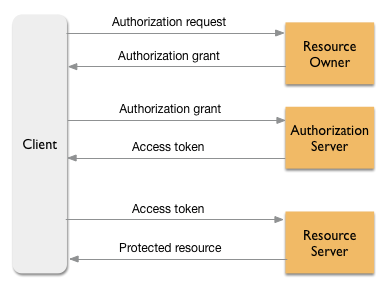
\includegraphics[width=0.85\textwidth]{images/oauth-abstract.png}
    \caption{Flusso di autorizzazione OAuth 2.0 \cite{oauth-image}}
    \label{fig:oauth-flow}
\end{figure}

\subsection{Piattaforme Fitbit e API disponibili}
Fitbit è una marca di dispositivi wearable, aquisita nel 2019 da Google \cite{fitbit}, che comprende una vasta gamma di prodotti i quali sono in grado di rilevare una grande quantità di dati.
Una volta che l'utente ha connesso il proprio dispositivo alla piattaforma Fitbit, è possibile utilizzare una serie di API che permettono di accedere a tali dati. La piattaforma Fitbit adotta lo standard OAuth 2.0 per l'autenticazione.
Tra i dati disponibili tramite le API Fitbit troviamo ad esempio:

\begin{itemize}
    \item Battito cardiaco
    \item Calorie bruciate
    \item Calorie assunte
    \item Ossigenazione del sangue
    \item Attività fisica
    \item Sonno
    \item Temperatura corporea
    \item Temperatura della pelle
    \item Attività respiratoria
\end{itemize}

e molti altri.
\\Una nota da precisare è che quasi tutti i dati sono disponibili in formato intraday(ossia visibuli con una frequenza che va da qualche secondo a pochi minuti), ma per accedere a questo livello di dettaglio è necessario mandare una richiesta speciale a Fitbit per entrare in possesso dell'autorizzazione necessaria alla loro consultazione \cite{fitbitapi}.

\subsection{Altre piattaforme e loro integrazione}

In commercio, oltre ai dispositivi Fitbit, esiste una vasta gamma di prodotti wearable per il monitoraggio dei parametri vitali con vari livelli di funzionalità: dai più economici ai più costosi. Tra questi possiamo trovare:

\begin{itemize}
    \item \textbf{Garmin Smartwatch}: Dispositivi molto avanzati dotati delle tecnologie più evolute per il monitoraggio. Molto adottati dagli sportivi. \cite{mysql}
    \item \textbf{Apple Watch}: Orologi smart progettati per un'integrazione perfetta con l'ecosistema Apple. L'accesso ai dati di tali dispositivi risulta più difficoltosa che su altre tipologie di dispositivi in quanto per ottenere l'accesso ai dati risulta necessario un dispositivo Apple. \cite{applewatch}
    \item \textbf{Amazfit}: Dispositivi la cui feature principale è il prezzo. Risultano infatti molto più competitivi (in linea generale) dal punto di vista economico rispetto ai dispositivi sopra citati. \cite{amazfit}
\end{itemize}



\chapter{Analisi dei requisiti}
Per l'analisi dei requisiti (funzionali e non funzionali) è stata utilizzata la metodologia MoSCoW \cite{moscow}, la quale permette di classificare i requisiti in quattro categorie: Must have (M), Should have (S), Could have (C) e Won't have (W).

\section{Requisiti funzionali}

\subsection{Autenticazione e sicurezza - M}

\begin{itemize}
    \item Il sistema deve fornire un meccanismo sicuro di registrazione per i medici e gli operatori sanitari.
    \item Gli utenti devono potersi autenticare tramite email e password.
    \item Il sistema deve supportare l'autenticazione API tramite token JWT.
    \item Le password devono essere memorizzate con crittografia sicura (libreria Werkzeug \cite{werkzeug}).
\end{itemize}

\subsection{Gestione pazienti - M}

\begin{itemize}
    \item I medici devono poter creare nuovi record paziente con informazioni anagrafiche di base.
    \item I medici devono poter visualizzare la lista di tutti i loro pazienti.
    \item I medici devono poter visualizzare i dettagli completi di un paziente.
    \item I medici devono poter modificare le informazioni dei loro pazienti.
    \item I medici devono poter aggiungere note mediche ai record dei pazienti
\end{itemize}

\subsection{Interfaccia Utente - M}

\begin{itemize}
    \item Il sistema deve fornire una dashboard per i medici che mostri statistiche rilevanti.
    \item L'interfaccia deve essere accessibile tramite browser web standard.
    \item L'interfaccia utente deve essere responsiva per supportare diversi dispositivi.
    \item La navigazione deve essere intuitiva e coerente in tutta l'applicazione.
\end{itemize}

\subsection{API Base - M}

\begin{itemize}
    \item Il sistema deve fornire API RESTful per le operazioni CRUD sui pazienti.
    \item Le API devono supportare la ricerca e il filtraggio dei pazienti.
    \item Le API devono essere protette tramite autenticazione JWT.
    \item Le risposte API devono seguire standard coerenti e gestire gli errori in modo appropriato.
\end{itemize}

\subsection{Integrazione con Piattaforme Sanitarie - S}

\begin{itemize}
    \item Il sistema dovrebbe integrarsi con Fitbit per recuperare dati sui parametri vitali.
    \item I medici dovrebbero poter visualizzare i parametri vitali del paziente in formato grafico.
    \item Il sistema deve supportare l'autenticazione API tramite token JWT.
    \item Il sistema dovrebbe supportare l'autenticazione OAuth con le piattaforme sanitarie.
\end{itemize}

\subsection{Osservazioni sui Parametri Vitali - S}

\begin{itemize}
    \item I medici dovrebbero poter creare osservazioni sui parametri vitali dei pazienti.
    \item I medici dovrebbero poter modificare e eliminare le loro osservazioni.
    \item Il sistema dovrebbe supportare diversi tipi di parametri vitali (frequenza cardiaca, pressione sanguigna, ecc.).
    \item Le osservazioni dovrebbero essere visualizzabili in modo cronologico.
\end{itemize}

\subsection{Internazionalizzazione - S}

\begin{itemize}
    \item L'interfaccia utente dovrebbe essere disponibile in italiano e inglese.
    \item Il sistema dovrebbe consentire agli utenti di cambiare facilmente lingua.
    \item Date e numeri dovrebbero essere formattati in base alle convenzioni locali.
    \item I messaggi di errore dovrebbero essere localizzati.
\end{itemize}

\subsection{Reportistica - S}

\begin{itemize}
    \item Il sistema dovrebbe generare report base sui dati dei pazienti.
    \item I report dovrebbero essere esportabili in formati standard (PDF).
    \item I report dovrebbero essere inviabili al paziente tramite email.
    \item I medici dovrebbero poter personalizzare alcuni parametri dei report.
    \item I report generati dovrebbero essere archiviati per consultazioni future.
\end{itemize}

\subsection{Integrazione con Ulteriori Piattaforme Sanitarie - C}

\begin{itemize}
    \item Il sistema potrebbe integrarsi con Apple Health.
    \item Il sistema potrebbe integrarsi con Google Fit.
    \item Il sistema potrebbe integrarsi con Garmin Connect.
    \item Il sistema potrebbe supportare dispositivi medici Bluetooth LE.
\end{itemize}

\subsection{Collaborazione tra Medici  - C}

\begin{itemize}
    \item I medici potrebbero condividere l'accesso ai pazienti con altri medici.
    \item Il sistema potrebbe supportare commenti collaborativi sulle note mediche.
    \item I medici potrebbero ricevere notifiche quando ci sono aggiornamenti sui pazienti condivisi.
    \item Il sistema potrebbe tenere traccia di chi ha effettuato modifiche ai record.
\end{itemize}

\subsection{Autenticazione a Due Fattori  - C}

\begin{itemize}
    \item Il sistema potrebbe supportare l'autenticazione a due fattori via SMS.
    \item Il sistema potrebbe supportare l'autenticazione a due fattori via app mobile.
    \item L'utente potrebbe configurare le preferenze di sicurezza del proprio account.
    \item Il sistema potrebbe richiedere 2FA per operazioni sensibili.
\end{itemize}

\subsection{Analisi Avanzata dei Dati  - C}

\begin{itemize}
    \item Il sistema potrebbe implementare algoritmi di rilevamento anomalie nei parametri vitali.
    \item Il sistema potrebbe offrire suggerimenti basati sui trend dei dati.
    \item Il sistema potrebbe generare report comparativi tra pazienti anonimi.
    \item Il sistema potrebbe supportare la visualizzazione di correlazioni tra diversi parametri.
\end{itemize}

\subsection{Prescrizione Elettronica - W}

\begin{itemize}
    \item Il sistema non supporterà la generazione di prescrizioni elettroniche.
    \item Non ci sarà integrazione con farmacie o sistemi di prescrizione nazionali.
    \item Non sarà possibile tracciare l'aderenza ai farmaci prescritti.
    \item Non ci sarà un modulo di gestione inventario farmaci.
\end{itemize}

\subsection{Cartella Clinica Elettronica Completa  - W}

\begin{itemize}
    \item Il sistema non sostituirà una cartella clinica elettronica completa.
    \item Non ci saranno moduli per la gestione di esami di laboratorio.
    \item Non ci sarà integrazione con sistemi ospedalieri.
    \item Non ci sarà supporto per la gestione di immagini diagnostiche.
\end{itemize}

\subsection{Telemedicina  - W}

\begin{itemize}
    \item Il sistema non includerà funzionalità di videoconferenza.
    \item Non ci sarà supporto per consultazioni remote in tempo reale.
    \item Non ci saranno strumenti per la pianificazione di visite virtuali.
    \item Non ci sarà integrazione con sistemi di pagamento per visite telematiche.
\end{itemize}

\subsection{App Mobile Dedicata  - W}

\begin{itemize}
    \item Non verrà sviluppata un'app mobile dedicata nella prima fase.
    \item I pazienti non avranno accesso diretto al sistema.
    \item Non ci sarà supporto per notifiche push su dispositivi mobili.
    \item Non ci sarà funzionalità offline per l'app mobile.
\end{itemize}


\section{Requisiti non funzionali}

\subsection{Sicurezza e Privacy - M}

\begin{itemize}
    \item Tutti i dati personali dei pazienti devono essere crittografati a riposo.
    \item Deve essere implementato un sistema completo di log per gli audit di sicurezza.
\end{itemize}

\subsection{Performance  - M}

\begin{itemize}
    \item Il tempo di risposta per le operazioni di base deve essere inferiore a 2 secondi.
    \item Il sistema deve supportare almeno 1000 utenti concorrenti.
    \item Il caricamento della dashboard non deve richiedere più di 3 secondi.
    \item Il sistema deve supportare la gestione di almeno 100.000 record paziente.
\end{itemize}

\subsection{Disponibilità  - M}

\begin{itemize}
    \item Il sistema deve avere un uptime del 99,9\% durante le ore lavorative.
    \item I backup del database devono essere eseguiti quotidianamente.
\end{itemize}

\subsection{Usabilità  - M}

\begin{itemize}
    \item L'interfaccia utente deve essere utilizzabile senza formazione specifica ed essere user-friendly.
    \item I flussi di lavoro principali non devono richiedere più di 3 clic.
    \item I messaggi di errore devono essere chiari e fornire indicazioni per la risoluzione.
\end{itemize}

\subsection{Scalabilità - S}

\begin{itemize}
    \item  L'architettura dovrebbe supportare lo scaling orizzontale.
    \item Il database dovrebbe gestire efficacemente l'aumento di volume dei dati.
    \item Le prestazioni non dovrebbero degradarsi significativamente con l'aumentare degli utenti.
    \item Il sistema dovrebbe implementare tecniche di caching per migliorare la reattività.
\end{itemize}

\subsection{Manutenibilità - S}

\begin{itemize}
    \item Il codice dovrebbe seguire standard di codifica e best practice.
    \item La documentazione del codice dovrebbe essere completa e aggiornata.
    \item L'architettura dovrebbe essere modulare per facilitare gli aggiornamenti.
    \item Il sistema dovrebbe supportare aggiornamenti con tempi di inattività minimi.
\end{itemize}

\subsection{Portabilità - S}

\begin{itemize}
    \item Il sistema dovrebbe funzionare sui principali browser web (Chrome, Firefox, Edge, Safari).
    \item L'interfaccia utente dovrebbe adattarsi a diverse risoluzioni dello schermo.
    \item Il sistema dovrebbe essere containerizzato per facilitare il deployment.
    \item Il backend dovrebbe funzionare su diversi sistemi operativi server.
\end{itemize}

\subsection{Interoperabilità - S}

\begin{itemize}
    \item Le API dovrebbero seguire standard RESTful.
    \item Il sistema dovrebbe supportare almeno il formato JSON per lo scambio di dati.
    \item Il sistema dovrebbe utilizzare formati standard per date, orari e dati medici.
\end{itemize}

\subsection{Prestazioni Avanzate - C}

\begin{itemize}
    \item Il sistema potrebbe implementare tecniche di precaricamento dei dati.
    \item L'interfaccia utente potrebbe utilizzare rendering lato server per il caricamento iniziale.
    \item Il sistema potrebbe implementare la compressione delle risposte API.
    \item Il database potrebbe essere ottimizzato con indici avanzati e strategie di partizionamento.
\end{itemize}

\subsection{Monitoraggio e Analytics - C}

\begin{itemize}
    \item Il sistema potrebbe implementare dashboard di monitoraggio in tempo reale.
    \item Le metriche di prestazione potrebbero essere raccolte e analizzate.
    \item Il sistema potrebbe implementare alerting automatico per problemi prestazionali.
    \item Gli errori utente potrebbero essere tracciati per identificare problemi di usabilità
\end{itemize}

\subsection{Supporto Offline - C}

\begin{itemize}
    \item L'interfaccia utente potrebbe implementare funzionalità progressive web app.
    \item I dati critici potrebbero essere memorizzati nella cache del browser.
    \item Il sistema potrebbe supportare la sincronizzazione dei dati dopo la riconnessione.
    \item Le modifiche potrebbero essere accodate quando offline.
\end{itemize}

\subsection{Testing Automatizzato - C}

\begin{itemize}
    \item Il sistema potrebbe avere una copertura di test unitari superiore all'85\%.
    \item Il sistema potrebbe implementare test di carico programmati.
    \item Il processo di CI/CD potrebbe includere test di sicurezza automatizzati.
\end{itemize}

\subsection{Supporto Legacy - W}

\begin{itemize}
    \item Non ci sarà compatibilità con sistemi operativi obsoleti.
    \item Non verranno fornite versioni desktop standalone.
\end{itemize}

\subsection{Alta Disponibilità Geografica - W}

\begin{itemize}
    \item Il sistema non implementerà il deployment multi-regione nella prima fase.
    \item Non ci sarà failover automatico tra diversi data center.
    \item Non ci sarà ottimizzazione per utenti in regioni geografiche specifiche.
    \item Non ci sarà un sistema di content delivery network globale.
\end{itemize}

\subsection{Integrazione Enterprise Completa - W}

\begin{itemize}
    \item Non ci sarà supporto per Single Sign-On aziendale completo.
    \item Non ci sarà integrazione con sistemi ERP legacy.
    \item Non ci saranno connettori personalizzati per ogni sistema clinico.
\end{itemize}

\subsection{Conformità Internazionale Completa - W}

\begin{itemize}
    \item Il sistema non sarà inizialmente certificato per standard internazionali come HIPAA.
    \item Non ci sarà supporto completo per tutti i requisiti normativi regionali.
    \item Non ci saranno localizzazioni complete per tutti i paesi.
    \item Non ci sarà certificazione FDA come dispositivo medico.

\end{itemize}

\section{Casi d'uso}
\subsection{Attori principali}
I principali attori del sistema risultano essere i medici e gli operatori sanitari, i quali si interfacciano con il sistema per la gestione dei pazienti e dei dati clinici.
I pazienti non hanno accesso diretto al sistema, ma possono comunque ricevere via email i report generati e sono necessari nel flusso di autenticazione necessario per concedere l'accesso dei proprio dati al sistema.
\subsection{Gestione dei pazienti}
I medici e gli operatori sanitari possono:
\begin{itemize}
    \item Visualizzare i pazienti.
    \item Creare nuovi pazienti.
    \item Importare pazienti tramite UUID.
    \item Visualizzare i dettagli di un paziente.
    \item Modificare i dettagli di un paziente.
    \item Eliminare un paziente(dissociandolo dal proprio account).
\end{itemize}
\subsection{Gestione dell'account}
I medici e gli operatori sanitari possono:
\begin{itemize}
    \item Registrare un nuovo account.
    \item Eseguire il login.
    \item Eseguire il logout.
\end{itemize}
\subsection{Visualizzazione dei parametri vitali}
I medici e gli operatori sanitari possono:
\begin{itemize}
    \item Visualizzare grafici dei parametri vitali.
    \item Visualizzare i parametri vitali in formato di tabelle.
    \item Selezionare un livello di dettaglio per la visualizzazione dei dati (1g, 7g, 30g, 90g).
\end{itemize}
\subsection{Gestione note}
I medici e gli operatori sanitari possono:
\begin{itemize}
    \item Creare nuove note cliniche.
    \item Visualizzare note esistenti.
    \item Eliminare note(solo quelle create da loro).
    \item Visualizzare i dettagli di un paziente.
    \item Modificare i dettagli di un paziente.
    \item Eliminare un paziente.
\end{itemize}
\subsection{Gestione report}
I medici e gli operatori sanitari possono:
\begin{itemize}
    \item Generare report specifici relativi ad un parametro vitale.
    \item Generare un report generale relativo a tutti i parametri vitali.
    \item Selezionare gli elementi(note, osservazioni, grafici) da includere nel report.
    \item Scaricare il report in formato PDF.
    \item Inviare una copia per email al paziente del report in formato PDF.
\end{itemize}
\subsection{Integrazione con piattaforme sanitarie}
I pazienti possono:
\begin{itemize}
    \item Autorizzare la connessione del proprio account alla piattaforma.
\end{itemize}
La piattaforma su cui sono salvati i dati può:
\begin{itemize}
    \item Revocare l'autorizzazione di accesso al sistema.
\end{itemize}
I medici e gli operatori sanitari possono:
\begin{itemize}
    \item Generare un link valido 24h per permettere all'utente di fornire l'accesso da parte della piattaforma ai suoi dati.
    \item Reimuovere il collegamento alla della piattaforma alla piattaforma su cui sono salvati i dati.
\end{itemize}
\subsection{Gestione delle osservazioni cliniche}
I medici e gli operatori sanitari possono:
\begin{itemize}
    \item Creare un'osservazione clinica relativa ad un parametro vitale e ad un periodo temporale specifico.
    \item Visualizzare le note esistenti per ciascun paziente.
    \item Eliminare un'osservazione clinica(solo quelle create da loro).
\end{itemize}



\section{User stories e scenari comuni principali}
\subsection{Registrazione e accesso}
\begin{itemize}
    \item Il medico o il personale sanitario accede al sistema collegandosi tramite un browser al link fornitogli.
    \item Si presentano due opzioni: registrazione e login.
    \item Per registrarsi l'utente clicca sul collegamento "Nuovo medico? Registrati Qui"(La lingua effettiva dipende dalla localizzazione selezionata).
    \item L'utente, seguendo le richieste specficate nella pagina, compila i campi con i propri dati, facendo attenzione a rispettare i requisiti di sicurezza della password.
    \item Se tutto è stato inserito correttamente, non esistono altri account nel sistema con la stessa email e il sistema non ha restituito errori, dopo aver premuto il pulsante "Crea Account" l'utente viene registrato e reindirizzato alla pagina di login.
    \item L'utente può accedere al sistema inserendo la propria email e password.
    \item L'utente, se i dati sono corretti e se il sistema non ha restituito errori, dopo aver premuto il pulsante "Accedi" viene reindirizzato alla Dashboard del sistema.
\end{itemize}
\subsection{Importazione e gestione pazienti}
\begin{itemize}
    \item Il medico o il personale sanitario accede e si trova davanti alla Dashboard.
    \item Decide di aggiungere un paziente: clicca sulla shortcut nella Dashboard "Nuovo Paziente" nel Menù Azioni rapide(oppure va nella pagina "Visualizza tutti i pazienti" e clicca sul pulsante "Aggiungi nuovo paziente").
    \item Nel form che si apre, l'utente compila i campi obbligatori richiesti e, se desidera, quelli opzionali.
    \item Dopo aver compilato il form, se i dati inseriti sono validi e se il sistema non ha restituito errori, dopo aver cliccato il pulsante "Salva Paziente" verrà creato un nuovo account.
    \item Dalla schermata "Visualizza tutti i pazienti" l'utente può importare un paziente esistente tramite UUID cliccando sul pulsante "Importa Paziente tramite UUID".
    \item Nel modale che si aprirà, l'utente inserirà il codice di associazione richiesto.
    \item Se il codice di associazione inserito è valido e associato ad un account paziente esistente (e se il sistema non ha restituito errori), dopo il click sul pulsante "Importa Paziente" il paziente verrà aggiunto alla lista dei pazienti seguiti dall'operatore.
\end{itemize}
\subsection{Collegamento dispositivi wearable}
\begin{itemize}
    \item Il medico o il personale sanitario accede e si trova davanti alla Dashboard.
    \item Decide di collegare un dispositivo wearable al profilo di un paziente: clicca sul pulsante "Visualizza tutti i pazienti" e, sulla lista dei pazienti, clicca sul pulsante Azione "Visualizza i parametri vitali".
    \item Nella pagina che si trova davanti, l'utente clicca sul pulsante "Health Sync".
    \item Viene aperto un modale che mostra un QR Code (per permettere ad un paziente in visita al medico di collegarsi scansionandolo) ed un link testuale che può essere condiviso con il paziente tramite email o messaggio.
    \item Il paziente, una volta ricevuto il link, cliccando su di esso viene reindirizzato alla pagina di autorizzazione all'accesso ai propri dati da parte del sistema, la quale può essere raggiungibile per 24h (o comunque fino a che la procedura di autorizzazione non sarà riuscita). Se il link non dovesse essere più valido il paziente verrà informato di questo.
    \item Il paziente clicca sul servizio relativo al dispositivo che possiede (inizialmente saranno supportati solo i dispositivi Fitvbit).
    \item Si apre la pagina di login della piattaforma scelta, la quale dopo aver effettuato l'accesso chiede all'utente di autorizzare una certa serie di permessi al sistema richiedente.
    \item Una volta concessi, l'utente viene reindirizzato alla pagina dei servizi disponibili e gli viene comunicato l'esito dell'operazione(fallita o riuscita).
    \item Il medico è ora collegato al dispositivo del paziente e può visualizzare i dati relativi ai parametri vitali nella schermata in cui ha cliccato "Health Sync".
\end{itemize}
\subsection{Visualizzazione e interpretazione dei dati}
\begin{itemize}
    \item Il medico o il personale sanitario accede e si trova davanti alla Dashboard.
    \item Clicca su "Visualizza tutti i pazienti" e clicca sull'azione "Visualizza Paziente".
    \item Qui il medico può intragire con le note relative al paziente, oltre che a visualizzare i relativi dati di registrazione.
    \item Clicca sul pulsante "Visualizza i parametri vitali" e si apre la pagina con i dati relativi al parametri vitali del paziente.
    \item Il medico, dopo che è stato effettuato il collegamento al dispositivo wearable, può visualizzare i dati relativi ai parametri vitali in formato tabellare o grafico.
    \item Il medico può decidere il livello di dettaglio di visualizzazione dei dati andando a cliccare sul pulsante relativo al periodo scelto(1g, 7g, 30g, 90g).
    \item Il medico può cambiare il parametro vitale visualizzato cliccando sulla voce relativa al parametro vitale desiderato.
\end{itemize}

\subsection{Generazione e invio report}
\begin{itemize}
    \item Il medico o il personale sanitario accede e si trova davanti alla Dashboard.
    \item Clicca su "Visualizza tutti i pazienti" e clicca sull'azione "Visualizza Parametri Vitali".
    \item Nella schermata che si apre, il medico visualizza i dati relativi ai parametri vitali del paziente.
    \item Nella sezione "Reports" il medico può scegliere di aprire la pagina di generazione del report relativa a tutti i parametri o a un singolo parametro vitale specifico.
    \item Se si sceglie su un parametro vitale specifico, la pagina verrà aperta con selezionato in automatico il grafico da includere nel report relativo al parametro vitale che era visualizzo nella pagina precedente(e con lo stesso livello di dettaglio).
    \item Se si sceglie su "Report Completo", la pagina verrà aperta con selezionati in automatico tutti i grafici relativi ai parametri vitali presenti(con il livello di dettaglio che era selezionato).
    \item In qualsiasi caso è possibile aggiungere o rimuovere parametri vitali e/o grafici. Inoltre è possibile aggiungere o rimuovere note cliniche e osservazioni cliniche.
    \item Il medico può inserire un messaggio opzionale riepilogativo con eventuali suggerimenti per il paziente.
    \item Il medico può selezionare di inoltrare una copia del report al paziente via email(solo se questa è stata inserita nel campo opzionale del paziente al momento della registrazione).
    \item Il medico cliccca su "Genera Report PDF" e una copia PDF del report verrà scaricata sul dispositivo.
    \item Se selezionata l'opzione di invio email, il sistema invierà una copia del report anche al paziente tramite email.
\end{itemize}

\subsection{Visualizzazione degli audit}
\begin{itemize}
    \item Il medico o il personale sanitario accede e si trova davanti alla Dashboard.
    \item Clicca sul pulsante "Visualizza i Log delle Attività" e sistema si apre la pagina con gli audit.
    \item Il medico visualizza una pagina con tutte le operazioni eseguite sugli utenti che esso segue (generati o importati) organizzate per "Azione" ed "Entità".
    \item Il medico può filtrare i dati per utente, Data(inizio e fine), tipo di azione, tipo di entità, paziente.
    \item Il medico può visualizzare dei grafici riepilogativi delle azioni eseguite in fondo alla pagina.
\end{itemize}

\subsection{Modifica dati personali}
\begin{itemize}
    \item Il medico o il personale sanitario accede e si trova davanti alla Dashboard.
    \item Clicca sul pulsante in alto a destra col proprio nome.
    \item Nella tendina che si apre clicca su "Profilo".
    \item Si apre una pagina con i suoi dati personali.
    \item Per modificare i propri dati, il medico aggiorna i campi contenenti i vecchi dati con quelli nuovi e, verificando che questi soddisfino la validazione, clicca su "Aggiorna Profilo" (per i dati normali) o "Aggiorna passato" (per la password).
    \item Se i dati inseriti sono validi e il sistema non ha restituito errori, il medico riceve un messaggio che lo informa dell'avvenuto aggiornamento dei suoi dati.
\end{itemize}

\chapter{Progettazione}
\section{Architettura del sistema}
\subsection{Architettura generale e componenti principali}
VitaLink è strutturata come un'applicazione web progettata per essere altamente scalabile e modulabile. Essa utilizza il Framework Flask (Python) per il backend, Bootstrap per il frontend e PostgreSQL come database relazionale(ma è possibile sostiturlo facilmente con un DBMS analogamente relazionale).
La piattaforma è progettata per essere inizialmente accessibile solo tramite browser web, ma sono state inserite anche delle API per permettere l'integrazione futura con possibili app mobile o altri sistemi esterni.
\subsection{Modularità e separazione delle responsabilità}
La piattaforma è divisa in 15 moduli principali, ai quali vanno ad affiancarsi due moduli di supporto per la gestione delle migrazioni e per la compilazione delle traduzioni al momento dell'istanziazione di un un container.
Vi sono poi le directory dei file static e dei template per quanto concerne il frontend, e la directory delle traduzioni per contenere le varie localizzazioni seguendo lo standard di Flask Babel.
Infine nella root del progetto è presente la cartella dei test. La cartella contiene inoltre un file di configurazione per la creazione di un ambiente e la fornitura di funzioni per la gestione dei test.
\begin{itemize}
    \item docs/ (cartella per la documentazione)
    \item app/
          \begin{itemize}
              \item static/ (cartella per i file statici, come CSS e JavaScript)
                    \begin{itemize}
                        \item css/ (cartella per i file CSS)
                              \begin{itemize}
                                  \item custom.css (file CSS personalizzato per lo stile dell'applicazione)
                                  \item health\_connect.css (file CSS specifico per lo stile della pagina di collegamento ai dispositivi)
                              \end{itemize}
                    \end{itemize}
                    \begin{itemize}
                        \item img/ (cartella per le immagini)
                              \begin{itemize}
                                  \item fitbit-logo.png (logo di Fitbit)
                                  \item apple-health-logo.png (logo di Apple Health)
                                  \item health-connect-logo.png (logo di Google Health Connect)
                              \end{itemize}
                    \end{itemize}
                    \begin{itemize}
                        \item js/ (cartella per i file JavaScript)
                              \begin{itemize}
                                  \item health\_platforms.js
                                  \item main.js
                                  \item observations.js
                                  \item patients.js
                                  \item specific\_report.js
                                  \item translations.js
                                  \item vital\_charts.js
                                  \item vitals.js
                              \end{itemize}
                    \end{itemize}
              \item templates/ (cartella per i template HTML)
                    \begin{itemize}
                        \item audit\_logs.html
                        \item base-no-session.html
                        \item base.html
                        \item dashboard.html
                        \item health\_connect\_result.html
                        \item health\_connect.html
                        \item login.html
                        \item patient\_detail.html
                        \item patients.html
                        \item patients.html
                        \item profile.html
                        \item register.html
                        \item specific\_report\_form.html
                        \item vitals.html
                    \end{itemize}
              \item translations/ (cartella per i file di traduzione)
                    \begin{itemize}
                        \item babel.cfg (file di configurazione per Babel)
                        \item messages.pot (file di template per le traduzioni)
                        \item it/ (cartella per le traduzioni in italiano)
                    \end{itemize}
              \item \_\_init\_\_.py
              \item app.py (modulo di configurazione per l'applicazione e il database)
              \item audit.py (modulo per la gestione dei log di audit)
              \item auth.py (modulo per la definizione delle autorizzazioni)
              \item compile\_translations.py (modulo per la compilazione delle traduzioni)
              \item email\_utils.py (modulo per l'integrazione del servizio di API per l'invio di email)
              \item health\_platforms\_config.py (modulo per la definizione delle API delle piattaforme sanitarie da cui recuperare i dati)
              \item health\_platforms.py (modulo per la configurazione del recupero dei dati dalle API definite in health\_platforms\_config.py)
              \item language.py (modulo per la gestione delle lingue)
              \item main.py (modulo punto di ingresso per l'applicazione)
              \item migrate.py (modulo per la gestione della migrazione del database. N.B che in caso di esecuzione locale è necessario configurare dapprima il database su psql andando a creare user, password, db e fornendo i permessi all'utente creato su tale db)
              \item models.py (modulo per la definizione dei modelli del database)
              \item observations.py (modulo per la gestione delle osservazionei cliniche)
              \item reports.py (modulo per la generazione dei report)
              \item utils.py (modulo per le funzioni di utilità)
              \item views.py (modulo controller per le viste web)
          \end{itemize}
    \item tests/
    \item Dockerfile (file di configurazione per la creazione dell'immagine Docker)
    \item docker-compose.yml (file di configurazione per la creazione e configurazione del container Docker)
    \item docker-entrypoint.sh (script di avvio del container Docker per la verifica della salute del DB)
    \item .env.example (file di esempio contenente la struttura necessaria per il settaggio dell'ambiente in ciascuna configurazione)
    \item .env (da configurare per sviluppo/test locale)
    \item db\_migrate.yml (script di migrazione per migrazione automatica in ambiente Docker)
    \item pyproject.toml (file di configurabilità per la gestione delle dipendenze e dei test)
    \item .dockerignore (file per escludere file e cartelle dalla creazione dell'immagine Docker)
    \item .gitignore (file per escludere file e cartelle dalla gestione di Git)
\end{itemize}
\subsection{Flusso dei dati e interazioni tra componenti}
Il frontend interagisce con il backend mediante richieste HTTP alle API RESTful della piattaforma, ricevendo risposte in formato JSON.
Queste API sono protette mediante autenticazione JWT o sessioni, facendo in modo che solo gli utenti autorizzati possano accedere ai dati. Il backend, implementato con Flask, gestisce tali richieste attraverso moduli specializzati come \texttt{auth.py} per l'autenticazione, \texttt{views.py} per le viste web e \texttt{api.py} per gli endpoint REST.
I dati rimangono immagazzinati nel database PostgreSQL, accessibile tramite l'ORM SQLAlchemy \cite{sqlalchemy} che astrae le interazioni a livello SQL.
Una componente chiave per l'obiettivo della piattaforma è il modulo \texttt{health\_platforms.py} che gestisce l'integrazione con servizi esterni come Fitbit mediante OAuth 2.0: quando un paziente autorizza l'accesso ai propri dati, il sistema riceve token di accesso e refresh che vengono memorizzati e associati al profilo dell'utente interessato.
Successivamente, il sistema può recuperare i dati sanitari chiamando le API esterne, elaborarli secondo le regole in \texttt{health\_platforms\_config.py} e memorizzarli temporaneamente nella cache per ottimizzare le prestazioni e ridurre le chiamate API (mitigando la possibilità di incorrere in blocchi).

\section{Design pattern}
Tra i pattern architetturali adottati nel progetto possiamo citare i più rilevanti.
\subsection{Pattern architetturali}
\begin{itemize}
    \item MVC (Model-View-Controller): separa la logica di business dalla presentazione, dell'interazione con la base di dati e della logica di controllo.
    \item Function Organization Pattern : ogni modulo è organizzato in funzioni, ciascuna delle quali ha una responsabilità specifica e coerente con la natura del modulo stesso.
\end{itemize}
\subsection{Pattern di progettazione}
\begin{itemize}
    \item Factory Pattern: utilizzato per creare oggetti in una superclasse, permettendo alle sottoclassi di alterare il tipo di oggetto creato.
    \item Strategy Pattern: permette di definire una famiglia di algoritmi incapsulati in classi separate.
    \item Decorator Pattern: permette di aggiungere responsabilità aggiuntive ad un oggetto senza modificarne la struttura.
\end{itemize}
\section{Modello dei dati}
Per il modello dei dati è stato scelto un'approccio relazionale in quanto non vi è una particolare necessità di un modello noSQL, essendo i dati sanitari di tipo strutturato e relazionabile.
\subsection{Entità principali e relazioni - Schema ER}
\begin{figure}[H]
    \centering
    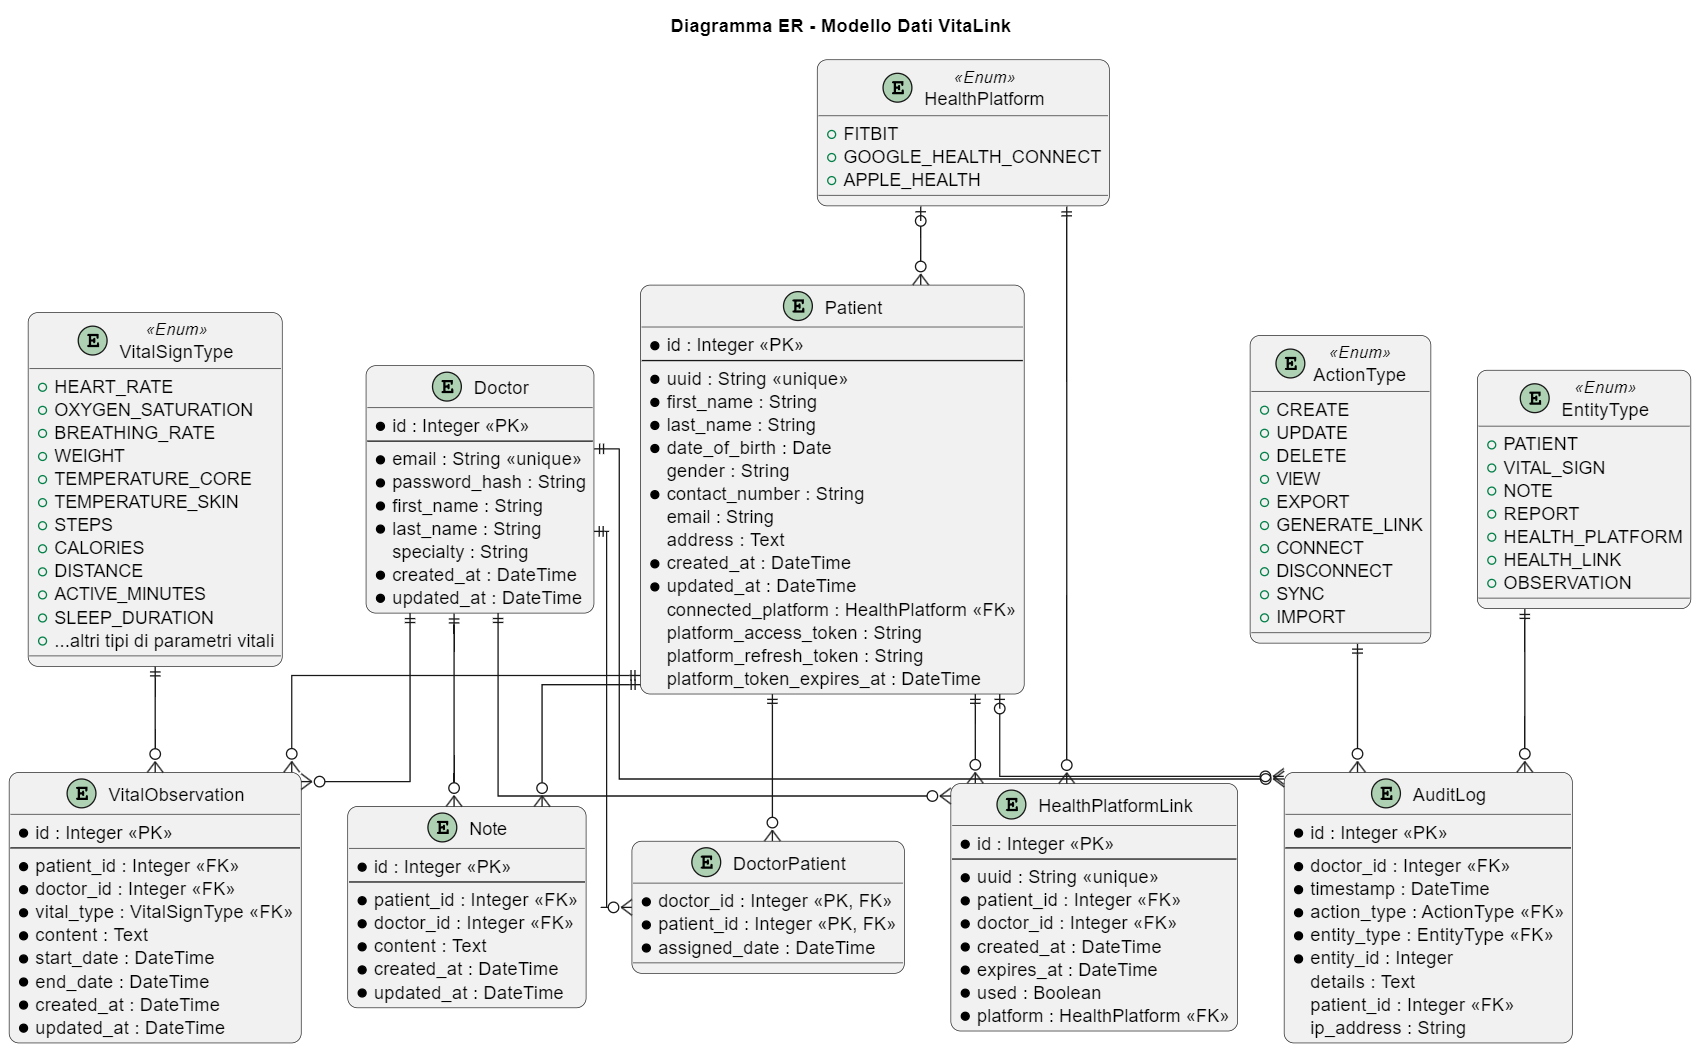
\includegraphics[width=0.85\textwidth]{images/DataModel.png}
    \caption{Schema ER completo del database}
    \label{fig:Schema-ER}
\end{figure}
\subsection{Enumerazioni e tipi di dati}
È stato scelto di utilizzare i tipi di dati standard di PostgreSQL per la definizione dei campi del database, in quanto sono sufficienti a soddisfare gli obiettivi perseguiti.
Sono presenti 4 Enum nel database utilizzati per casi specifici per garantire l'integrità dei dati e limitare i valori possibili ad un insieme predefinito di costanti.
\begin{itemize}
    \item Tipi di parametri vitali
    \item Tipo di piattaforma sanitaria
    \item Tipo di attività per l'audit
    \item Tipo di entità per l'audit
\end{itemize}
\section{Architettura del database}
È stato scelto PostgreSQL come DBMS relazionale in quanto risulta essere uno dei più diffusi e supportati dalle piattaforme per il deployment.
Non è comunque esclusa la possibilità di poter riconfigurare il sistema per l'utilizzo di un altro DBMS relazionale, come ad esempio MySQL o Microsoft SQL Server.
\subsection{Schema relazionale}
Per ovvie ragioni s
\subsection{Strategia di migrazione}

\section{Interfaccia utente}
\subsection{Design responsivo e mobile-first}
\subsection{Componenti UI per la visualizzazione dei dati sanitari}
\subsection{Flow di navigazione}

\section{API e integrazione con sistemi esterni}
\subsection{RESTful API design}
\subsection{Integrazione OAuth con Fitbit}
\subsection{Sistema di caching temporaneo}
\subsection{Estendibilità per future piattaforme}





\chapter{Implementazione}
\section{Stack tecnologico}
\subsection{Backend: Python e Flask}
\subsection{ORM: SQLAlchemy}
\subsection{Frontend: HTML5, CSS3, JavaScript}
\subsection{Database: PostgreSQL}
\subsection{Containerizzazione: Docker}

\section{Struttura del codice}
\subsection{Organizzazione dei moduli}
\subsection{Struttura dei package}
\subsection{Convenzioni di codifica}

\section{Implementazione del backend}
\subsection{Modelli di dati e ORM}
\subsection{Autenticazione e gestione degli utenti}
\subsection{Implementazione delle API RESTful}
\subsection{Sistema di audit e logging}
\subsection{Integrazione con piattaforme sanitarie}
\subsection{Gestione delle osservazioni cliniche}

\section{Implementazione del frontend}
\subsection{Struttura delle pagine e componenti}
\subsection{Visualizzazione dei parametri vitali con grafici}
\subsection{Form per la gestione dei dati}
\subsection{Interfaccia per la generazione di report}

\section{Integrazione con API esterne}
\subsection{Flusso OAuth 2.0 per Fitbit}
\subsection{Gestione dei token e refresh}
\subsection{Recupero e processamento dei dati}
\subsection{Gestione degli errori e rate limiting}

\section{Sicurezza e autenticazione}
\subsection{Protezione degli endpoint}
\subsection{Gestione delle sessioni}
\subsection{JWT per autenticazione API}
\subsection{Logging di sicurezza e audit}





\chapter{Testing e Validazione}
\section{Strategia di testing}
\subsection{Approccio al testing}
\subsection{Ambienti di test}
\subsection{Automazione dei test}

\section{Unit testing}
\subsection{Test dei modelli}
\subsection{Test delle API}
\subsection{Test dei servizi}
\subsection{Mock e fixture}

\section{Integration testing}
\subsection{Test del flusso OAuth}
\subsection{Test del sistema di report}
\subsection{Test dell'integrazione con il database}

\section{User testing}
\subsection{Metodologia}
\subsection{Raccolta feedback}
\subsection{Risultati e miglioramenti}

\section{Validazione dei requisiti}
\subsection{Verifica dei requisiti funzionali}
\subsection{Analisi dei requisiti non funzionali}
\subsection{Completezza della soluzione}





\chapter{Deployment e Operations}
\section{Ambiente di deployment}
\subsection{Architettura dell'ambiente di produzione}
\subsection{Configurazione del server}
\subsection{Gestione delle variabili d'ambiente}

\section{Containerizzazione e orchestrazione}
\subsection{Docker e Docker Compose}
\subsection{Immagini e configurazione}
\subsection{Persistenza dei dati}

\section{Continuous Integration e Continuous Deployment}
\subsection{Pipeline CI/CD}
\subsection{Automazione dei test}
\subsection{Deployment automatizzato}

\section{Monitoraggio e logging}
\subsection{Strategia di logging}
\subsection{Monitoraggio delle performance}
\subsection{Gestione degli errori in produzione}





\chapter{Risultati e valutazione}
\section{Obiettivi raggiunti}
\subsection{Funzionalità implementate}
\subsection{Conformità ai requisiti}
\subsection{Innovazioni apportate}

\section{Metriche di performance}
\subsection{Tempo di risposta}
\subsection{Scalabilità e carico}
\subsection{Efficienza nell'uso delle risorse}

\section{Feedback degli utenti}
\subsection{Metodologia di raccolta feedback}
\subsection{Analisi delle risposte}
\subsection{Aree di miglioramento identificate}

\section{Limiti e problemi riscontrati}
\subsection{Sfide tecniche}
\subsection{Limitazioni delle API esterne}
\subsection{Compromessi di design}





\chapter{Conclusioni e sviluppi futuri}
\section{Conclusioni}
\subsection{Riepilogo del lavoro svolto}
\subsection{Contributi principali}
\subsection{Riflessione sul processo di sviluppo}

\section{Sviluppi futuri}
\subsection{Integrazione con ulteriori piattaforme sanitarie}
\subsection{Funzionalità avanzate di analisi predittiva}
\subsection{Espansione del sistema di reportistica}
\subsection{Applicazione mobile companion}

\section{Considerazioni personali}
\subsection{Apprendimenti chiave}
\subsection{Sfide personali}
\subsection{Valore aggiunto dell'esperienza}

% Appendici
\appendix

\chapter{Glossario}
\begin{description}
    \item[API] Application Programming Interface
    \item[CI/CD] Continuous Integration/Continuous Deployment
    \item[JWT] JSON Web Token
    \item[MVC] Model-View-Controller
    \item[OAuth 2.0] Protocollo di autorizzazione standard dell'industria
    \item[ORM] Object-Relational Mapping
    \item[REST] Representational State Transfer
    \item[UI] User Interface
    \item[UML] Unified Modeling Language
    \item[UUID] Universally Unique Identifier
          % Aggiungere altri termini rilevanti
\end{description}

\chapter{Codice sorgente significativo}
\section{Modelli di dati}
\section{Autenticazione e sicurezza}
\section{Integrazione OAuth}
\section{Sistema di osservazioni}
\section{Generazione report}

\chapter{Diagrammi UML}
\section{Diagrammi dei casi d'uso}
\section{Diagrammi delle classi}
\section{Diagrammi di sequenza}
\section{Diagrammi di stato}
\section{Diagrammi delle attività}
\section{Diagrammi di deployment}
\section{Diagrammi ER}

% Bibliografia
\begingroup
\begin{thebibliography}{99}
    \bibitem{msd2025} MSD, Salute. (2025, January 23). \textit{Telemedicina. Ocse: "Raddoppiato il suo uso dopo la pandemia"}. MSD Salute. \url{https://msdsalute.it/approfondimenti/notizie/telemedicina-ocse-raddoppiato-il-suo-uso-dopo-la-pandemia/}
    \bibitem{anastasio2023} Anastasio, P. (2023, February 8). \textit{Sanità digitale, Italia in ritardo. 'Serve collaboration e telemedicina.'}. Key4biz. \url{https://www.key4biz.it/sanita-digitale-italia-ancora-indietro-puntare-su-collaboration-e-telemedicina/434361/}
    \bibitem{validic} \textit{An EHR-integrated solution for remote patient care}. (n.d.). Validic. \url{https://www.validic.com/}
    \bibitem{humanapi} \textit{What is Human API?} (n.d.). Human API. \url{https://reference.humanapi.co/docs/overview}
    \bibitem{withings} \textit{Health Mate by Withings - La migliore app per monitorare la tua attività, peso e altro}. (n.d.). Withings. \url{https://www.withings.com/it/it/health-mate}
    \bibitem{mywellness} SPA, T. (n.d.). \textit{mywellness}. \url{https://www.mywellness.com/cloud/}
    \bibitem{wellmo} Wellmo Mobile Wellness Solutions MWS Oy. (2025, May 6). \textit{Platform and mobile app for personalised digital health services}. Wellmo. \url{https://www.wellmo.com/}
    \bibitem{liva} \textit{Improving lives through digital health coaching | LiVA Healthcare}. (n.d.). \url{https://www.livahealthcare.com/}
    \bibitem{doccla} \textit{Doccla – Europe's leading virtual care solution}. (n.d.). \url{https://www.doccla.com/}
    \bibitem{geeksforgeeks} GeeksforGeeks. (2024, December 10). \textit{Top 7 Backend development Frameworks [2025 Updated]}. GeeksforGeeks. \url{https://www.geeksforgeeks.org/frameworks-for-backend-development/}
    \bibitem{bootstrap} Contributors, M. O. J. T. a. B. (n.d.). \textit{Bootstrap}. \url{https://getbootstrap.com/}
    \bibitem{flutter} \textit{Flutter - Build apps for any screen}. (n.d.) \url{https://flutter.dev/}
    \bibitem{react} \textit{React}. (n.d.). \url{https://react.dev/}
    \bibitem{GDPR} Altalex, R. (2019, February 22). \textit{GDPR - Regolamento generale sulla protezione dei dati}. Altalex. \url{https://www.altalex.com/documents/codici-altlex/2018/03/05/regolamento-generale-sulla-protezione-dei-dati-gdpr}
    \bibitem{mysql} \textit{MySQL}. (n.d.). \url{https://www.mysql.com/it/}
    \bibitem{postgresql} PostgreSQL. (2025, May 7). \textit{PostgreSQL}. \url{https://www.postgresql.org/}
    \bibitem{mongodb} \textit{MongoDB: the world’s leading modern database}. (n.d.). MongoDB. \url{https://www.mongodb.com/}
    \bibitem{bluetooth} \textit{Bluetooth App development: The role of Bluetooth in wearable technology | By Summer Swann | Connected Devices | Yeti LLC}. (n.d.). \url{https://www.yeti.co/blog/bluetooths-role-in-wearable-technology}
    \bibitem{ble} contributori di Wikipedia. (2025, March 21). \textit{Bluetooth Low energy}. Wikipedia. \url{https://it.wikipedia.org/wiki/Bluetooth_Low_Energy}
    \bibitem{ant} contributori di Wikipedia. (2022, March 8). \textit{ANT+}. Wikipedia. \url{https://it.wikipedia.org/wiki/ANT%2B}
    \bibitem{fitbit} contributori di Wikipedia. (2024, April 15). \textit{Fitbit}. Wikipedia. \url{https://it.wikipedia.org/wiki/Fitbit}
    \bibitem{fitbitapi} \textit{Fitbit Development: Intraday}. (n.d.). \url{https://dev.fitbit.com/build/reference/web-api/intraday/}
    \bibitem{garmin} \textit{Smartwatch | Orologi per lo Sport | GARMIN}. (n.d.). \url{https://www.garmin.com/it-IT/c/wearables-smartwatches/}
    \bibitem{applewatch} Apple. (n.d.). \textit{Apple Watch}. Apple (Italia). \url{https://www.apple.com/it/watch/}
    \bibitem{amazfit} amazfit-it. (2025, April 30). \textit{Amazfit Italia | Negozio online ufficiale}. Amazfit-it. \url{https://it.amazfit.com/}
    \bibitem{moscow} contributori di Wikipedia. (2024, September 5). \textit{Metodo MOSCOW}. Wikipedia. \url{https://it.wikipedia.org/wiki/Metodo_MoSCoW}
    \bibitem{werkzeug} \textit{Werkzeug — Werkzeug Documentation (3.1.x)}. (n.d.). \url{https://werkzeug.palletsprojects.com/en/stable/}
    \bibitem{oauth-image} Google Cloud. (n.d.). \textit{Flusso di autorizzazione OAuth 2.0}. Google Cloud Apigee. \url{https://cloud.google.com/static/apigee/docs/api-platform/images/oauth-abstract.png}
    \bibitem{sqlalchemy} SQLAlchemy. (n.d.). \url{https://www.sqlalchemy.org/}
\end{thebibliography}
\end{document}